% \ifthenelse{\boolean{iclr}}
% {
% \begin{figure}[htbp]
%     \centering
%     \begin{tcblisting}{
%     listing only, 
%     halign=left,
%     listing engine=minted,
%     minted language=python,
%     minted options={%
%         linenos,
%         breaklines,
%         autogobble,
%         fontsize=\footnotesize,
%         numbersep=2mm,
%         baselinestretch=1},
%     % title=\textbf{\small IterGen code for SQL generation},
%     colbacktitle=blue!30!white, 
%     coltitle=black,
%     left=0pt,               
%     right=0mm,              
%     top=0mm,                
%     bottom=0mm,             
%     boxsep=1mm,
%     width=\textwidth,
%     listing options={style=pythonstyle},
% }
% def generate_sql_with_itergen(iter_gen, problem):
%     iter_gen.start(problem['prompt'])
%     schema = parse_sql_schema(problem)
%     attempts = 0  

%     while not iter_gen.finished() and attempts < max_iter:
%         out = iter_gen.forward(stop_symbols=['column_name', 'table_name'])
%         attempts += 1 

%         if not exists_column(schema, iter_gen.view('column_name')[-1]):
%             iter_gen.backward('column_name')
%             continue

%         if not exists_table(schema, iter_gen.view('table_name')[-1]):
%             iter_gen.backward('table_name')
%             continue

%     return out
% \end{tcblisting}
%     \caption{Code using \Tool{} for LLM-based SQL Generation}
%     \label{fig:sql_algo}
% \end{figure}
% }
% {
\begin{figure}[htbp]
\centering
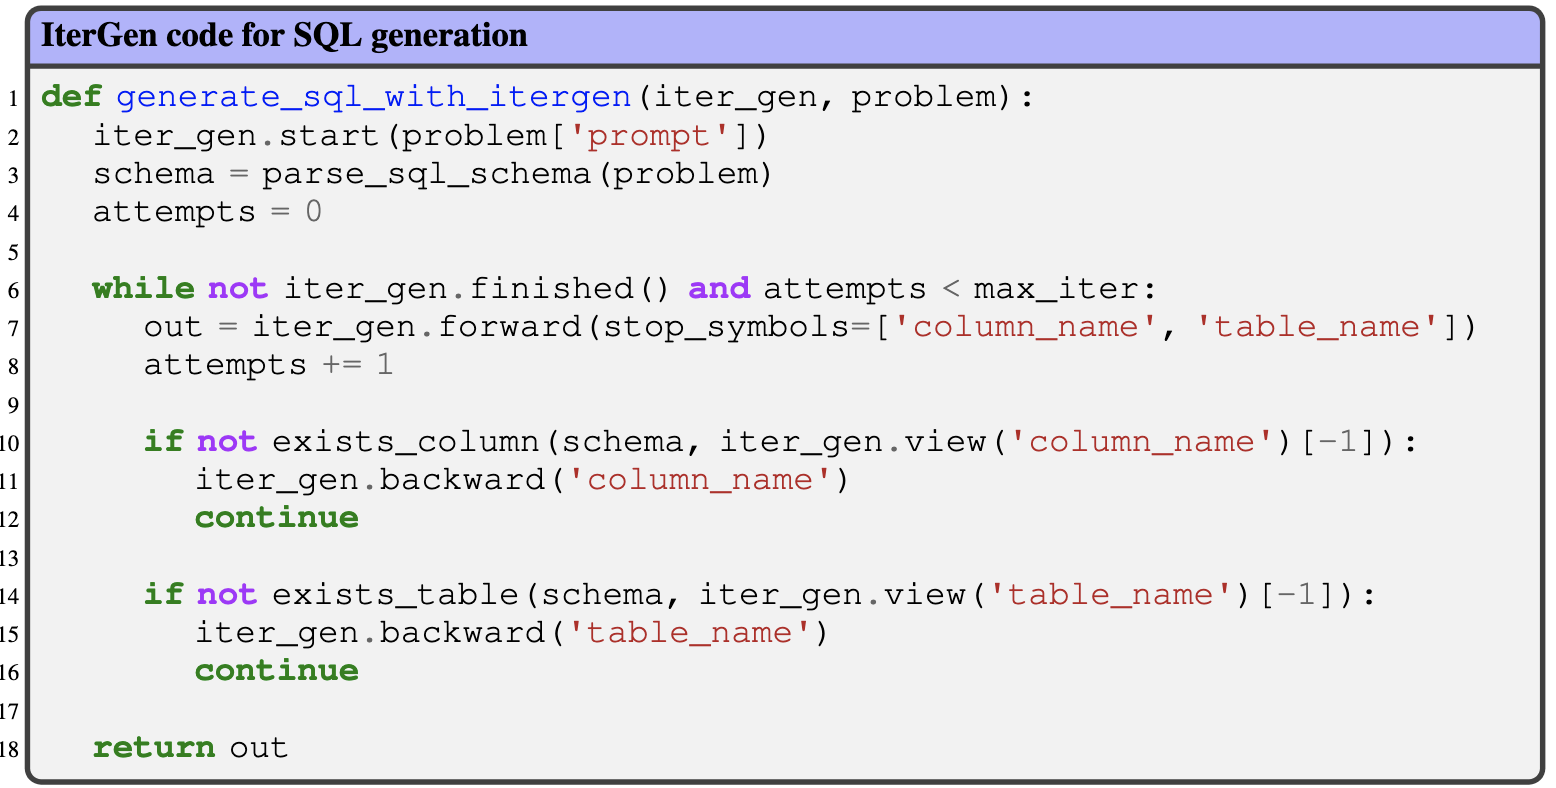
\includegraphics[width=\textwidth]{images/sql_code.png}
\caption{Code using \Tool{} for LLM-based SQL Generation}
\label{fig:sql_algo}
\end{figure}
% }

    